\chapter{Risk Propagation}

\NewDocumentCommand{\pr}{mo}{\IfNoValueTF{#2}{p(#1)}{p_{#2}(#1)}}
\NewDocumentCommand{\eventSpace}{}{\Omega}
\NewDocumentCommand{\event}{}{\omega}

%Refer to \Cref{sec:conventions} for the typographical conventions used in this chapter.

Risk propagation is a message-passing algorithm that estimate's an individual's infection risk by considering their demographics, symptoms, diagnosis, and contact with others. Formally, a \define{risk score} $\vScore_\vTime$ is a timestamped infection probability where $\vScore \in [0, 1]$ and $\vTime \in \naturals$ is the timestamp of its computation. Thus, an individual with a high risk score implies that they are likely to test positive for the disease and pose a significant health risk to others. There are two types of risk scores: \define{symptom scores}, or prior infection probabilities, which account for non-contact risk (e.g., demographics, symptoms, diagnosis) \cite{Menni2020}; and \define{exposure scores}, or posterior infection probabilities, which incorporate the risk introduced by interacting with others, either directly or indirectly.



Computing an individual's MPIP from the joint infection probability distribution scales exponentially with the size of the population. Moreover, requiring 

Marginalization the joint infection probability distribution is intractable as it scales exponentially with the number of individuals. To circumvent this challenge, risk propagation 

variation of message passing on a factor graph

To circumvent this challenge, risk propagation uses a variation of message passing on a factor graph. Formally, let $\vGraph = (\vVariables, \vFactors, \vEdges)$ be a factor graph where $\vVariables$ is the set of variable vertices, $\vFactors$ is the set of factor vertices, and $\vEdges$ is the set of edges incident between them \cite{Kschischang2001}. A \define{variable vertex} $\vVariable[i]$ is a random variable such that $\vVariable[i]: \eventSpace \rightarrow \{0, 1\}$, where the sample space is $\eventSpace = \{\var{healthy}, \var{infected}\}$ and
%
\begin{equation*}
    \vVariable[i](\event) =
        \begin{cases}
            0 & \text{if } \event = \var{healthy} \\
            1 & \text{if } \event = \var{infected}.
        \end{cases}
\end{equation*}
%
Thus, $\pr{\vVariable[i]}[\vTime] = \vScore_\vTime$ is a risk score of individual $i$. A \define{factor vertex} $\vFactor(\vVariable[i], \vVariable[j])$,  also denoted as $\vFactor[ij]$, represents contact between individuals $i, j$ such that $\vFactor[ij]$ is adjacent to $\vVariable[i], \vVariable[j]$. \Cref{fig:factor-graph} depicts a factor graph that reflects the problem constraints. Unlike the max-sum algorithm that aims to maximize the \emph{joint} distribution \cite[pp. 411--415]{Bishop2006}, the objective of risk propagation is to maximize \emph{individual} marginal probabilities \cite{Ayday2021}.
%
\begin{figure}[htbp]
    \centering
    \begin{tikzpicture}[ampersand replacement=\&]
    	\matrix[row sep=1.5em, column sep=0.75em]
    	{
    		\& \factor[minimum size=1em] {f12} {above:$\vFactor[12]$} {} {}; \&\&
    		\factor[minimum size=1em] {f23} {above:$\vFactor[23]$} {} {}; \& \\
    		\node[latent, minimum size=2em] (v1) {$\vVariable[1]$}; \&\&
    		\node[latent, minimum size=2em] (v2) {$\vVariable[2]$}; \&\&
    		\node[latent, minimum size=2em] (v3) {$\vVariable[3]$}; \\
    	};
    	\edge[-] {v1} {f12};
    	\edge[-] {v2} {f12};
    	\edge[-] {v2} {f23};
    	\edge[-] {v3} {f23};
    \end{tikzpicture}
    \caption[Factor graph]{A factor graph of 3 variable vertices and 2 factor vertices.}
    \label{fig:factor-graph}
\end{figure}

\section{System Models} % TODO

%\footnotetext{While previous work on ShareTrace \cite{Ayday2021} defines a \emph{contact} as a contiguous 15 minutes in which the devices of two users are proximal, the Centers for Disease Control and Prevention technically considers these 15 minutes \emph{over a 24-hour time window} \cite{CDC2021}.}

The system model is similar to that in previous work \cite{Ayday2020, Ayday2021}. \Cref{fig:actor-dataflow} illustrates the corresponding data flow\footnote{A \emph{data-flow diagram} consists of data processors (circles), directed data flow (arrows), data stores (parallel lines), and external entities (rectangles) \cite[pp. 437--438]{Fowler2004}\label{foot:dataflow}.}.
%
\begin{itemize}
    % TODO A more formal set of definitions for distributed, co-located, centralized, and decentralized computing is in order.
    % TODO More conceptual detail should be introduced before this point. Add a section in the Introduction that defines self-sovereignty concepts.
    \item Each user owns a \emph{personal data store} (PDS), a form of cloud storage that empowers the user with ownership and access control over their data.
    \item Symptom scores are computed in a user's PDS to support integrating multiple streams of personal data \cite{Ayday2020}. While local symptom-score computation \cite{Ayday2020, Ayday2021} is more privacy-preserving, it is assumed that the user's PDS is a trusted entity.
    \item User device interactions serve as a proxy for proximal human interactions. This work does not assume a specific protocol, but does assume that the protocol can approximate the duration of contact with relative accuracy and that communication with the actors of those contacted users can be established in a privacy-preserving manner.
    \item No geolocation data is collected \cite{Ayday2020}. As a decentralized, proximity-based solution, it is not necessary to collect user geolocation data. See \Cref{sec:location-based} for a discussion of a geolocation-based design that was considered.
    \item Actor-based risk propagation is a distributed, online algorithm \cite[pp. 791--818]{Cormen2022}. Previous work \cite{Ayday2020, Ayday2021} (see also \Cref{sec:previous-designs}) formulates risk propagation as a centralized, offline algorithm that periodically aggregates all user data to estimate infection risk. To improve the privacy, scalability, and responsiveness of ShareTrace, this work designs risk propagation to avoid data aggregation and to estimate infection risk in near real-time.
\end{itemize}

\begin{figure}[htb]
    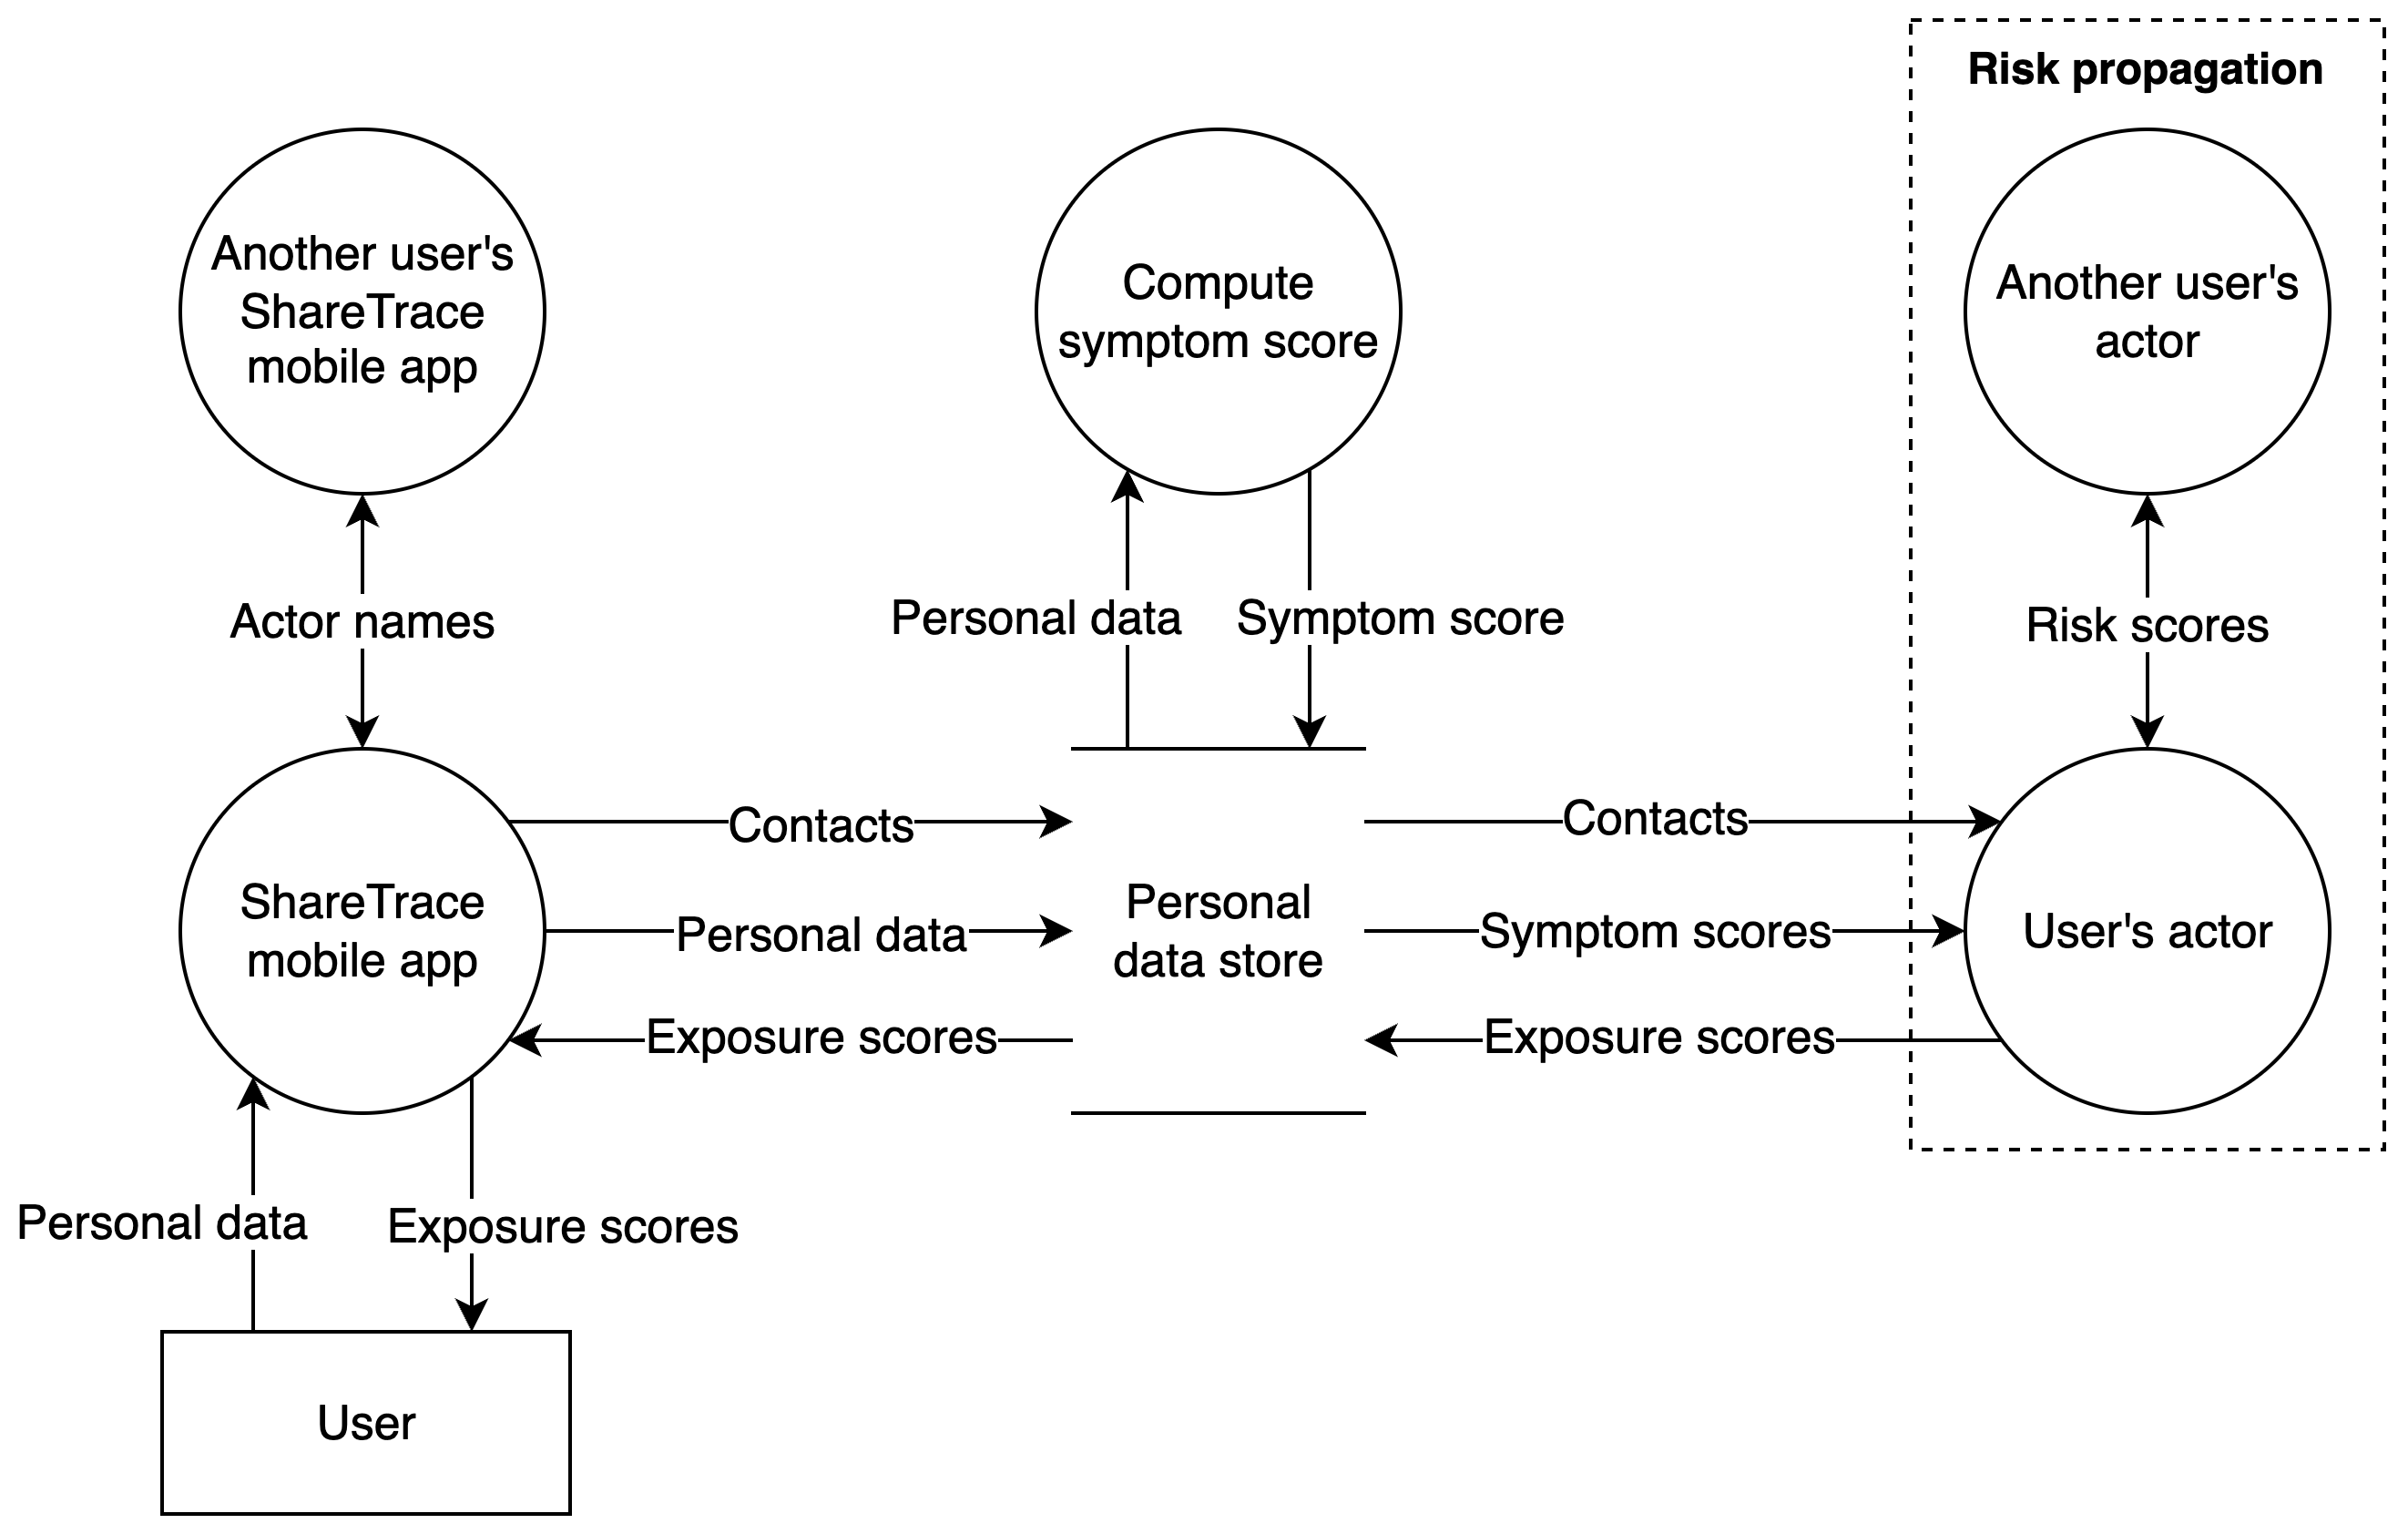
\includegraphics[width=\textwidth]{distributed-dataflow}
    \caption[Distributed ShareTrace data flow]{Distributed ShareTrace data flow. \emph{Contacts} include the actor name and contact time of all users with which the user came into close proximity. \emph{Personal data} includes the user's demographics, reported symptoms, and diagnosis. It may also include machine-generated biomarkers and electronic health record data \cite{Ayday2020}.}
    \label{fig:distributed-dataflow}
\end{figure}

\begin{figure}[htb]
    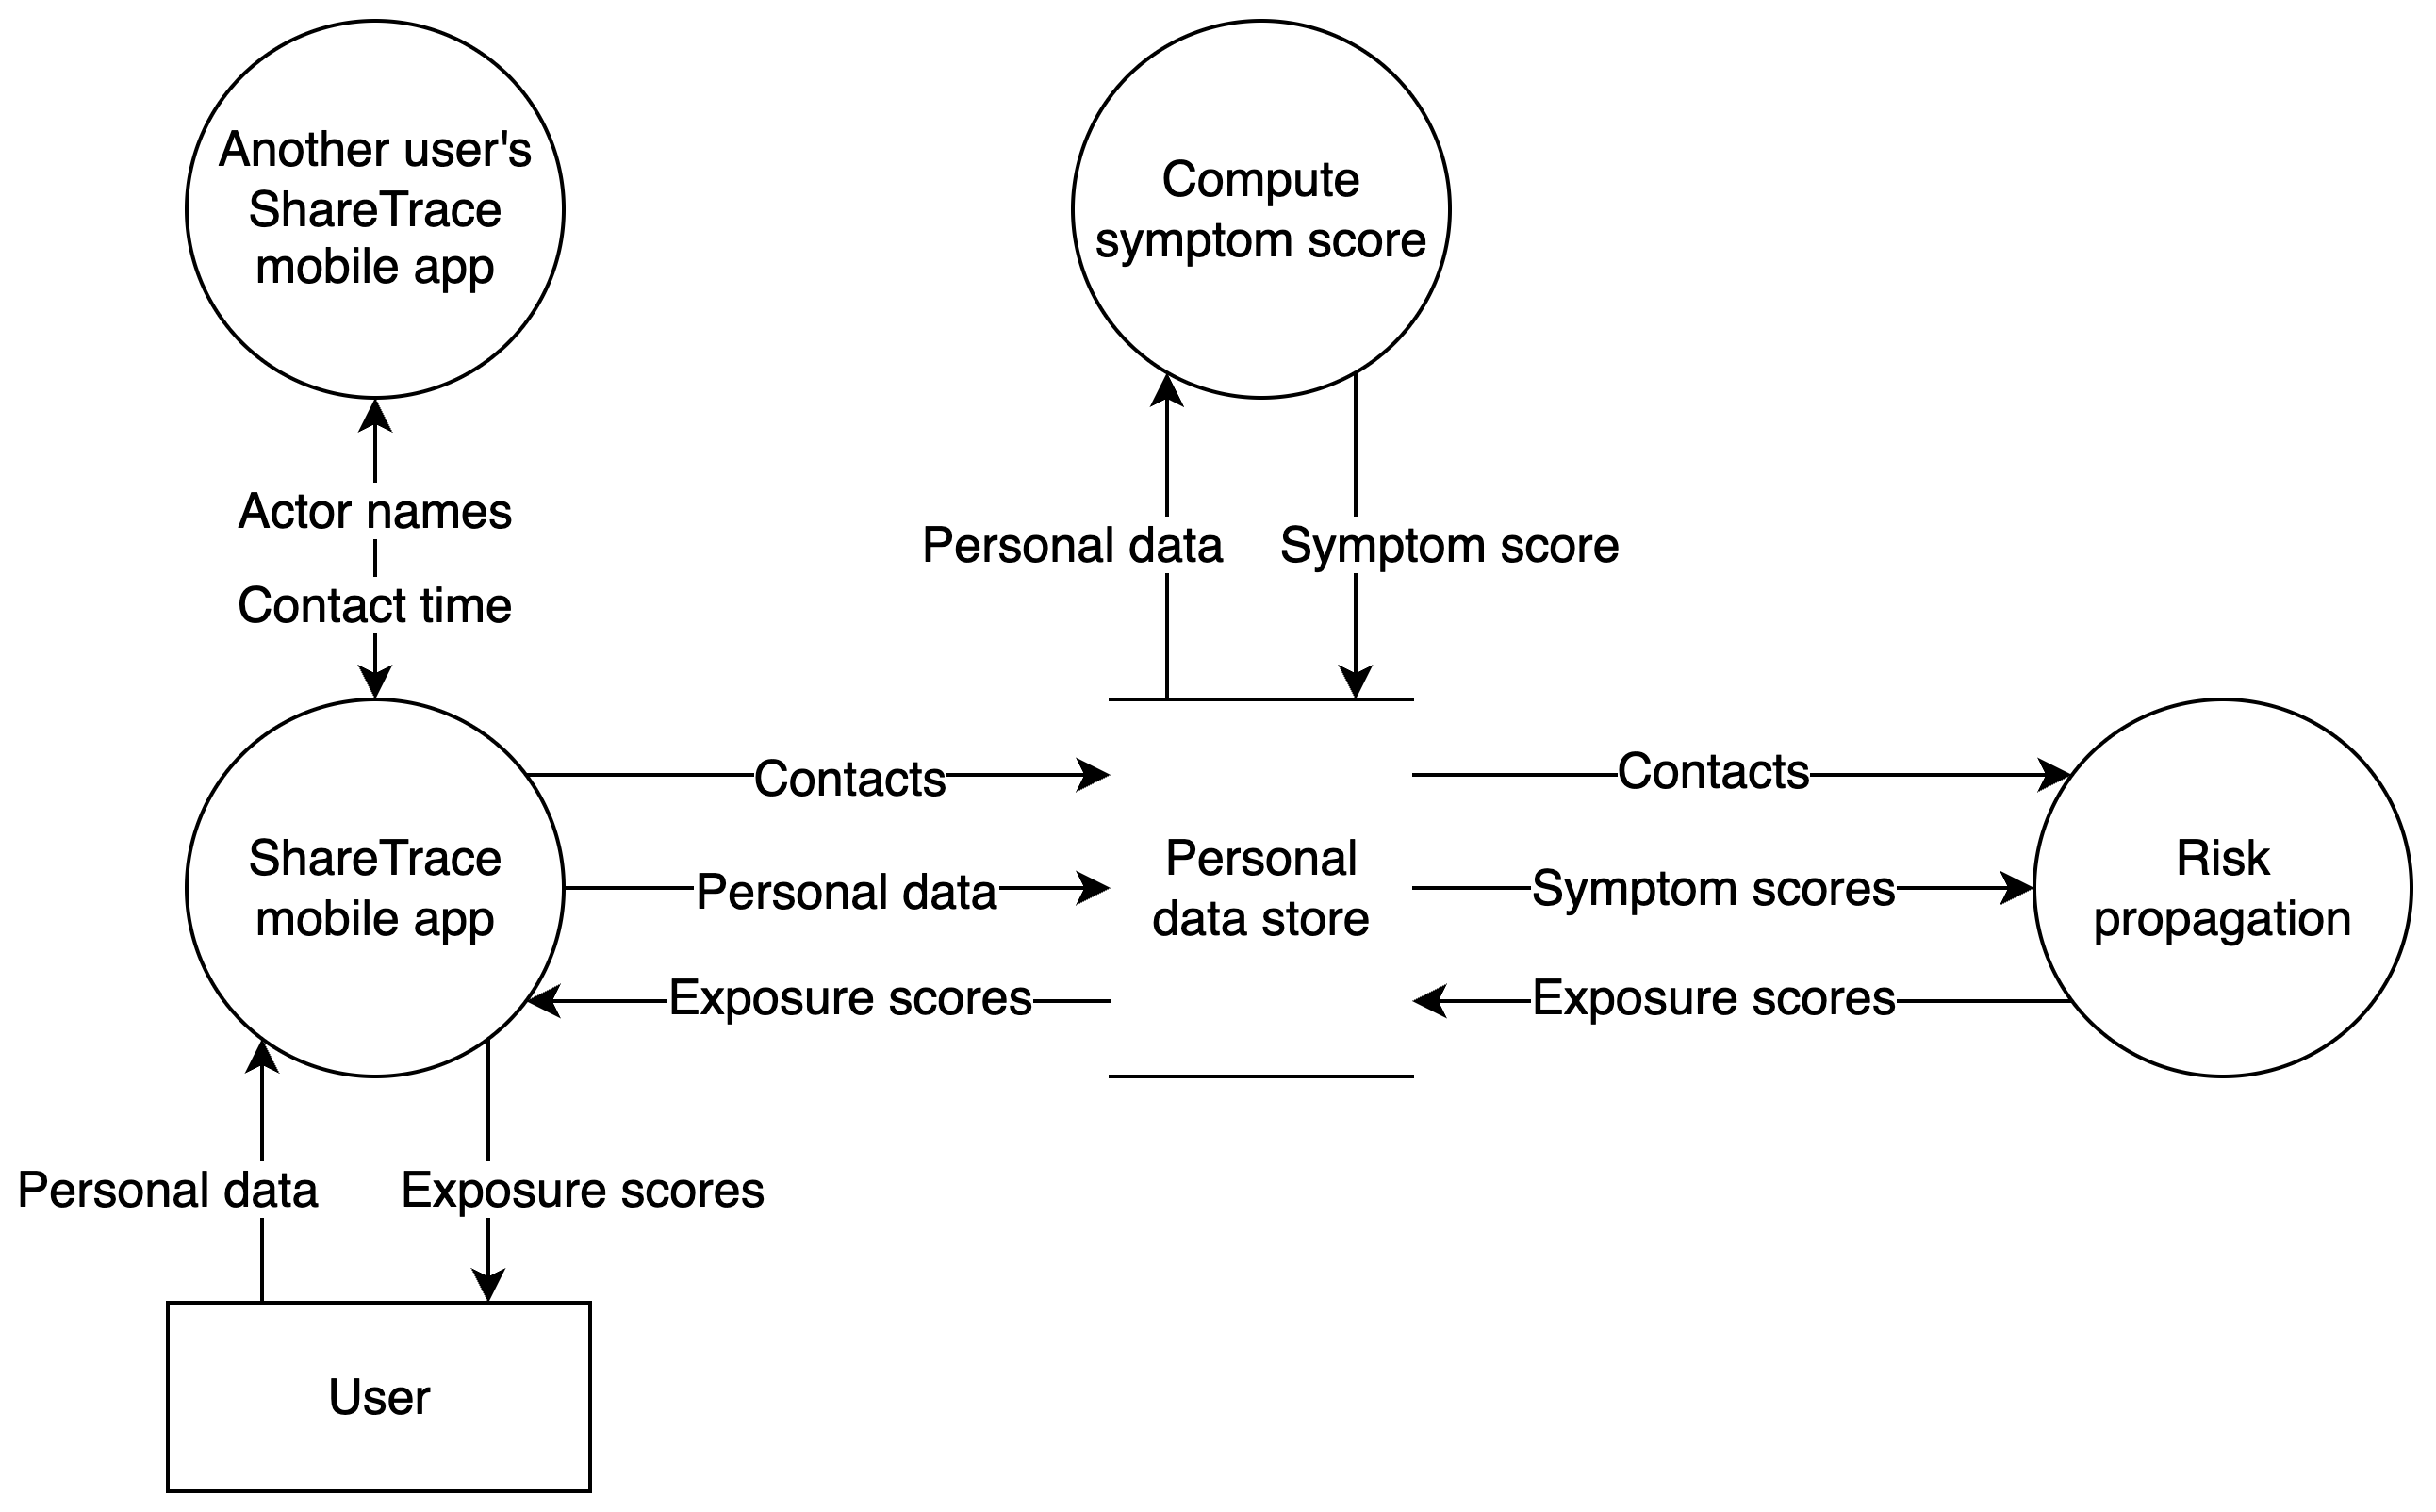
\includegraphics[width=\textwidth]{centralized-dataflow}
    \caption[Centralized ShareTrace data flow]{Centralized ShareTrace data flow. \emph{Contacts} include the actor name and contact timestamp of all users with which the user came into close proximity. \emph{Personal data} includes the user's demographics, reported symptoms, and diagnosis. It may also include machine-generated biomarkers and electronic health record data \cite{Ayday2020}.}
    \label{fig:centralized-dataflow}
\end{figure}

\section{Synchronous Risk Propagation}

\NewDocumentCommand{\diff}{o}{\IfNoValueTF{#1}{\delta}{\delta_{#1}}}
\NewDocumentCommand{\topK}{m}{\text{top } K \text{ of } #1}
\NewDocumentCommand{\scores}{mm}{R_{#1}^{(#2)}}

%Risk propagation was originally defined as an iterative message-passing algorithm in which the message passing was performed directly on the factor graph that was derived from the ShareTrace user population.\cite{Ayday2021}. Moreover, the termination condition
%
%- iteration = global strate, offline, centralized
%
%As a basis for defining non-iterative versions of the algorithm, this section covers iterative risk propagation. With the exception of a few improvements, the definition provided in this section is identical to that provided in previous work \cite{Ayday2021}. Specifically, iterative risk propagation is an offline algorithm that requires centralized aggregation of individuals' risk scores and contacts. 
%
%Note that the description of iterative risk propagation in this section does not assume a particular model of computation. In fact, the notion of a ``message'' in the following description need not correspond to a literal message that is passed during execution.

\begin{function}[H]{\nSyncRiskProp}[S, C; \pTransRate, \pTimeBuffer, K, N, \diff]
\State $(\vVariables, \vFactors, \vEdges) \assign \Call{Factor-Graph}{C}$
\State $n \assign 1$
\State $\diff[n -1] \assign \infty$
\ForEach{$\vVariable[i] \in \vVariables$}
	\State $\scores{i}{n - 1} \assign \topK{S_i}$
\EndFor
\While{$n \leq N \AND \diff[n - 1] > \diff$}
	\ForEach{$\{\vVariable[i], \vFactor[ij]\} \in \vEdges$}
		\State $\vVariableMsg{i}{ij}{n} \assign \scores{i}{n - 1} \setminus \setbuilder{\vFactorMsg{ij}{i}{k}}{k \in [1 \ltwodots n - 1]}$
	\EndFor
	\ForEach{$\{\vVariable[i], \vFactor[ij]\} \in \vEdges$}
		\State $\vFactorMsg{ij}{j}{n} \assign \max (\{0\} \cup \setbuilder{\pTransRate \cdot \vScore_\vTime}{\vScore_\vTime \in \vVariableMsg{i}{ij}{n}, \vTime < \vTime_{ij} + \pTimeBuffer})$
	\EndFor
	\ForEach{$\vVariable[i] \in \vVariables$}
		\State $\scores{i}{n} \assign \topK{\setbuilder{\vFactorMsg{ij}{i}{k}}{k \in [1 \ltwodots n], \vFactor[ij] \in \neighbors_i}}$
	\EndFor
	\State $\diff[n] \assign 0$
	\ForEach{$\vVariable[i] \in \vVariables$}
		\State $\diff[n] \assign \diff[n] + \max \scores{i}{n} - \max \scores{i}{n - 1}$
	\EndFor
	\State $n \assign n + 1$
\EndWhile
\State \Return $\setbuilder{\max \scores{i}{n}}{\vVariable[i] \in \vVariables}$
\end{function}

\section{Asynchronous Risk Propagation}\label{sec:vertices-to-actors}

The only purpose of a factor vertex is to compute and relay messages between variable vertices. Thus, one-mode projection onto the variable vertices can be applied such that variable vertices $\vVariable[i],\vVariable[j] \in \vVariables$ are adjacent if the factor vertex $\vFactor[ij] \in \vFactors$ exists \cite{Zhou2007}. \Cref{fig:projected} shows the modified topology.
%
\begin{figure}[htbp]
\centering
\begin{tikzpicture}[ampersand replacement=\&]
	\matrix[row sep=7em, column sep=2em]
	{
		\node[latent, minimum size=2em] (v1) {$\vVariable[1]$}; \&\&\&
		\node[latent, minimum size=2em] (v2) {$\vVariable[2]$}; \&\&\&
		\node[latent, minimum size=2em] (v3) {$\vVariable[3]$}; \\
	};
	\factor[minimum size=1em, above= of v1] {f12_1} {above:$\vFactor[12]$} {} {};
	\factor[minimum size=1em, above= of v2, xshift=-3em] {f12_2} {above:$\vFactor[12]$} {} {};
	\factor[minimum size=1em, above= of v2, xshift=3em] {f23_2} {above:$\vFactor[23]$} {} {};
	\factor[minimum size=1em, above= of v3] {f23_3} {above:$\vFactor[23]$} {} {};

	\plate{p1} {(v1)(f12_1)(f12_1-caption)} {};
	\plate{p2} {(v2)(f12_2)(f23_2)(f12_2-caption)(f23_2-caption)} {};
	\plate{p3} {(v3)(f23_3)(f23_3-caption)} {};

	\edge[-] {v1} {f12_1};
	\edge[-] {v2} {f12_2};
	\edge[-] {v2} {f23_2};
	\edge[-] {v3} {f23_3};
	\edge[-] {p1} {p2};
	\edge[-] {p2} {p3};
\end{tikzpicture}
\caption[One-mode projection of a factor graph]{One-mode projection
onto variable vertices of \Cref{fig:factor-graph}. While the projected graph
contains only variable vertices, the original factor vertices are also included
to show how the original topology is modified.}
\label{fig:projected}
\end{figure}
%
To send a message to variable vertex $\vVariable[i]$, variable vertex $\vVariable[j]$ applies the computation associated with the factor vertex $\vFactor[ij]$. This modification differs from the distributed extension of risk propagation \cite{Ayday2021} in that we do not create duplicate factor vertices and messages in each user's PDS. By storing the contact time between users on the edge incident to their variable vertices, this modified topology is identical to the \emph{contact-sequence} representation of a \emph{contact network}, a kind of \emph{time-varying} or \emph{temporal network} in which a vertex represents a person and an edge indicates that two persons came in contact:

\begin{equation}
    \setbuilder{(\vVariable[i], \vVariable[j], \vTime)}{\vVariable[i], \vVariable[j] \in \vVariables; \vVariable[i] \neq \vVariable[j]; \vTime \in \naturals}, \label{eq:contact-seq}
\end{equation}
%
where a triple $(\vVariable[i], \vVariable[j], \vTime)$ is called a \emph{contact} \cite{Holme2012}. Specific to risk propagation, $\vTime$ is the time at which users $u$ and $v$ \emph{most recently} came in contact (see \Cref{sec:vertices-to-actors}).

The usage of a temporal network in this work differs from its typical usage in epidemiology which focuses on modeling and analyzing the spreading dynamics of disease \cite{Riolo2001, Danon2011, Lokhov2014, Craft2015, Pastor-Satorras2015, Koher2019, Zino2021}. In contrast, this work uses a temporal network to infer a user's MPPI. As a result, \Cref{sec:reachability} extends temporal reachability to account for both the message-passing semantics and temporal dynamics of the network. As noted by \cite{Holme2012}, the transmission graph provided by \cite{Riolo2001} ``cannot handle edges where one vertex manages to not catch the disease.'' Notably, the usage of a temporal network in this work allows for such cases by modeling the possibility of infection as a continuous outcome.
% TODO
Factor graphs are useful for decomposing complex probability distributions and allowing for efficient inference algorithms.

However, as with risk propagation, and generally any application of a factor graph in which the variable vertices represent entities of interest (i.e., of which the marginal probability of a variable is desired), applying one-mode projection is a .

\subsection{ShareTrace Actor System}

As a distributed algorithm, risk propagation is specified from the perspective of an \emph{actor}, which is equivalent to the paradiagm of \emph{think- like-a-vertex} graph-processing algorithms \cite{McCune2015}. Some variation exists on exactly how actor behavior is defined \cite{AghaThesis1985, Agha1985, Koster2016}. Perhaps the simplest definition is that the \emph{behavior of an actor} is both its \emph{interface} (i.e., the types of messages it can receive) and \emph{state} (i.e., the internal data it uses to process messages) \cite{Koster2016}. An \emph{actor system}\footnote{This is technically referred to as an \emph{actor system configuration}.} is defined as the set of actors it contains and the set of unprocessed messages\footnote{Formally, a \emph{message} is called a \emph{task} and is defined by a \emph{tag}, a unique identifier; a \emph{target}, the mail address to which the message is delivered; and a \emph{communication}, the message content \cite{AghaThesis1985}.} in the actor mailboxes. An expanded definition of an actor system also includes a \emph{local states function} that maps mail addresses to behaviors, the set of \emph{receptionist actors} that can receive communication that is external to the actor system, and the set of \emph{external actors} that exist outside of the actor system \cite{AghaThesis1985, Agha1985}. Practically, a local states function is unnecessary to specify, so the narrower definition of an actor system is used. The remainder of this section describes the components of the ShareTrace actor system.

\subsubsection{User Actor Behavior}\label{sec:behavior}

Each user corresponds to an actor that participates in the message-passing protocol of risk propagation. Herein, the user of an actor will only be referred to as an \emph{actor}. The following variant of the concurrent, object-oriented actor model is assumed to define actor behavior \cite{Agha1985, Agha1990}.
%
\begin{itemize}
	\item An actor follows the \emph{active object pattern} \cite{Lavender1996, Koster2016} and the \emph{Isolated Turn Principle} \cite{Koster2016}. Specifically, the state change of an actor is carried out by instance- variable assignment, instead of the canonical \cBecome{} primitive that provides a functional construct for pipelining actor behavior replacement \cite{AghaThesis1985, Agha1985, Agha1990}. The interface of a user actor is fixed in risk propagation, so the more general semantics of \cBecome{} is unnecessary.
	\item The term ``name'' \cite{Hewitt1977, AghaThesis1985} is preferred over ``mail address'' \cite{AghaThesis1985, Agha1985, Agha1990} to refer to the sender of a message. Generally, the mail address that is included in a message need not correspond to the actor that sent it. Risk propagation, however, requires this actor is identified in a risk-score message. Therefore, to emphasize this requirement, ``name'' is used to refer to both the identity of an actor and its mail address.
	\item An actor is allowed to include a loop with finite iteration in its behavior definition; this is traditionally prohibited in the actor model \cite{AghaThesis1985, Agha1990}.
	\item Because the following pseudocode to describe actor behavior mostly follows the conventions of \cite{Cormen2022} (see \Cref{sec:conventions}), the behavior definition is implied by all procedures that take as input an actor.
\end{itemize}
%
The \cCreateActor{} operation initializes an actor, which is equivalent to the \emph{new expression} \cite{AghaThesis1985} or \cCreate{} primitive \cite{Agha1985, Agha1990} with the exception that it only specifies the attributes (i.e., state) of an actor. As mentioned earlier, the behavior description of an actor is implied by the procedures that require an actor as input. Every actor $\vActor$ has the following attributes.
%
\begin{itemize}
	\item $\aActorName$: an identifier that enables actors to communicate with it \cite{Hewitt1977, AghaThesis1985}.
	\item $\aActorContacts$: a dictionary (see \Cref{sec:conventions}) that maps an actor name to a timestamp. That is, if user $i$ of actor $\vActor_i$ comes in contact with user $j$ of actor $\vActor_j$, then the \emph{\nContactsAttr} of $\vActor_i$ contains the name of $\vActor_j$ along with the most recent contact time for users $i$ and $j$. The converse holds for user $j$. This is an extension of the \emph{acquaintance vector} \cite{Hewitt1977} or \emph{acquaintance list} \cite{AghaThesis1985, Agha1985}.
	\item $\aActorScore$: the user's current exposure score. This attribute is either a default risk score (see \cDefaultScore), a risk score sent by an actor of some contacted user\footnote{As discussed later (see \cHandleContactMessage{} in \Cref{sec:behavior}), it possible for an actor $i$ to send a message to an actor $j$ but not be a contact of actor $j$.}, or a symptom score of the user.
	\item $\aActorCache$: a dictionary that maps a time interval to a risk score; used to tolerate synchronization delays between a user's device and actor (see \Cref{sec:caching}).
\end{itemize}
%
\begin{function}{\nCreateActor}
    \State $\aActorName \assign \cCreateName$
    \State $\aActorContacts \assign \emptyset$
    \State $\aActorScore \assign \cDefaultScore[\vActor]$
    \State $\aActorCache \assign \emptyset$
    \State \Return $\vActor$
\end{function}
% TODO Default risk score = placeholder and querying; never sent
% TODO Define a risk score as a message
\begin{function}{\nDefaultScore}[\vActor]
    \State $\aScoreValue \assign 0$
    \State $\aScoreTime \assign 0$
    \State $\aScoreSender \assign \aActorName$
    \State \Return $\vScore$
\end{function}
%
Risk scores and contacts have finite relevance, which is parametrized by a \emph{liveness} or \emph{relevance duration} $\pScoreTtl, \pContactTtl > 0$, respectively. The relevance of risk scores and contacts is important, because it influences how actors pass messages. For example, actors do not send irrelevant risk scores or relevant risk scores to irrelevant contacts. The \emph{time-to-live} (TTL) of a risk score or contact is the remaining duration of its relevance. In the following operations, $\aScoreTime$ denotes the time at which the risk score was originally computed, $\aContactTime$ is the contact time, and \cGetTime{} returns the current time.
%
% TODO Define risk score and contact notation and standard attributes
\begin{function}{\nScoreTtl}[\vScore]
    \State \Return $\max \{0, \pScoreTtl - (\cGetTime - \aScoreTime)\}$
\end{function}
\begin{function}{\nContactTtl}[\vContact]
    \State \Return $\max \{0, \pContactTtl - (\cGetTime - \aContactTime)\}$
\end{function}
%
The interface of a user actor is defined by two types of messages: contact messages and risk-score messages. A \emph{contact message} $\vContact$ contains the name $\aContactName$ of the actor whose user was contacted and the contact time $\aContactTime$. A \emph{risk-score message} $\vScore$ is simply a risk score along with the actor's name $\aScoreSender$ that sent it. A risk score previously defined as the ordered pair $(\vScoreValue, \vTime)$ (see \Cref{sec:vertices-to-actors}) is represented as the attributes $\vScoreValue$ and $\aScoreTime$. The following sections discuss how a contact message and risk-message are processed by an actor.

\paragraph{Handling Contact Messages}\label{sec:contact-message-handling}

There are two ways in which a user actor can receive a contact message. The first, technically correct approach is for a receptionist actor to mediate the communication between the user actor and the PDS so that the user actor can retrieve its user's contacts. The second approach is to relax this formality and allow the user actor to communicate with the PDS directly\footnote{If the PDS itself is an actor, then a push-oriented dataflow could be implemented, where the user actor receives contact messages (and symptom-score messages). This would be more efficient and timely than a pull-oriented dataflow in which the PDS is a passive data store that requires the user actor or receptionist to poll it for new data.}.

The \cHandleContactMessage operation defines how a user actor processes a contact message. A contact is assumed to have finite relevance which is parametrized by the \emph{contact time-to-live} $\pContactTtl > 0$. A contact whose contact time occurred no longer than $\pContactTtl$ time ago is said to be \emph{alive}. Thus, a user actor only adds a contact if it is alive.
%
% TODO In practice, the two actors could establish trusted communication to
% avoid adding contacts the user did not actually come into contact with. Perhaps
% also requiring the Bluetooth ID received at the time of contact?
\begin{function}{\nHandleContactMessage}[\vActor, \vContact]
    \If{$\cContactTtl[\vContact] > 0$}
    	\State $\aContactKey \assign \aContactName$
    	\State $\aContactThreshold \assign 0$
    	\State $\cInsert[\aActorContacts, \vContact]$
    	\State $\cStartContactsRefreshTimer[\vActor]$
    	\State $\cSendCurrentOrCached[\vActor, \vContact]$
    \EndIf
\end{function}
%
\begin{function}{\nStartContactsRefreshTimer}[\vActor]
    \State $\vOldest \assign \cMinimum[\aActorContacts]$
    \If{$\vOldest \notEquals \nil$}
    	\State $\aTimerKey \assign \text{``contacts''}$
    	\State $\cStartTimer[\vTimer, \cContactTtl[\vOldest]]$
    \EndIf
\end{function}
%
\begin{function}{\nHandleContactsRefreshTimer}[\vTimer]
    \ForEach{$\vContact \in \aActorContacts$}
    	\If{$\cContactTtl[\vContact] \leq 0$}
    		\State $\cDelete[\aActorContacts, \vContact]$
    	\EndIf
    \EndFor
    \State $\cStartContactsRefreshTimer[\vActor]$
\end{function}
%
Regardless of whether the contact is alive, the user actor attempts to send a risk-score message that is derived from its current exposure score or a cached risk score (see \Cref{sec:caching}):
%
\begin{function}{\nSendCurrentOrCached}[\vActor, \vContact]
    \If{$\cShouldReceive[\vContact, \aActorScore]$} \label{step:send-current}
    	\State $\cSend[\vActor, \vContact, \aActorScore]$
    \Else
    	\State $\vScore \assign \cCacheMax[\aActorCache, \aContactTime + \pTimeBuffer]$ \label{step:cache-max}
    	\If{$\vScore \notEquals \nil \AND \cScoreTtl[\vScore] > 0$}
    		\State $\cSend[\vActor, \vContact, \vScore]$
    	\EndIf
    \EndIf
\end{function}
%
\begin{function}{\nSend}[\vActor, \vContact, \vScore]
    \State $\aSentScoreValue \assign \pTransRate \cdot \aScoreValue$
    \State $\aSentScoreTime \assign \aScoreTime$
    \State $\aSentScoreSender \assign \aActorName$
    \State $\cSend[\vContact, \vSentScore]$
    \State $\cUpdateThreshold[\vContact, \vSentScore]$
\end{function}
%
\begin{function}{\nShouldReceive}[\vContact, \vScore]
    \State \Return $\aContactThreshold < \aScoreValue \AND \aContactTime + \pTimeBuffer \geq \aScoreTime \AND \cScoreTtl[\vScore] > 0 \AND \aContactName \notEquals \aScoreSender$
\end{function}
%
\begin{function}{\nUpdateThreshold}[\vContact, \vScore]
    \State $\var{threshold} \assign \pSendCoeff \cdot \aScoreValue$
    \If{$\var{threshold} > \aContactThreshold}$
    	\State $\aContactThreshold \assign \var{threshold}$
    	\State $\cStartThresholdTimer[\vContact, \vScore]$
    \EndIf
\end{function}
%
\begin{function}{\nStartThresholdTimer}[\vContact, \vScore]
    \State $\aTimerKey \assign \aContactName + \text{`` threshold''}$
    \State $\aTimerName \assign \aContactName$
    \State $\cStartTimer[\vTimer, \cScoreTtl[\vScore]]$
\end{function}
%
\begin{function}{Handle-Threshold-Timer}[\vActor, \vTimer]
    \State $\vContact \assign \cSearch[\aActorContacts, \aTimerName]$
    \If{$\vContact \notEquals \nil$}
    	\State $\vScore \assign \cCacheMax[\aActorCache, \aContactTime + \pTimeBuffer]$
    	\If{$\vScore \notEquals \nil \AND \cScoreTtl[\vScore] > 0$}
    		\State $\aContactThreshold \assign \pSendCoeff \cdot \aScoreValue$
    		\State $\cStartThresholdTimer[\vContact, \vScore]$
    	\Else
    		\State $\aContactThreshold \assign 0$
    	\EndIf
    \EndIf
\end{function}
%
Like contacts, each risk score is assumed to have finite relevance that is parametrized by the \emph{score time-to-live} $\pScoreTtl > 0$ and evaluated by the operation \Call{Is-Score-Alive}{}. To send an actor's current exposure score, the contact must be sufficiently recent. It is assumed that risk scores computed after a contact occurred have no effect on the user's exposure score.

To account for the disease incubation period, a delay in reporting symptoms, or a delay in establishing actor communication, a time buffer $\pTimeBuffer \geq 0$ is considered. That is, a risk score is not sent to a contact if \Call{Is-Contact-Recent}{} returns \false.

The \Call{Transmitted}{} operation is used to generate risk scores that are sent to other actors. It is assumed that contact only implies an incomplete transmission of risk between users. Thus, when sending a risk score to another actor, the value of the risk score is scaled by the \emph{transmission rate} $\pTransRate \in (0, 1)$. Notice that the time of the risk score is left unchanged; the act of sending a risk-score message is independent of when the risk score was first computed.

If line \ref{step:send-current} of \cSendCurrentOrCached[] evaluates to \false, then the actor attempts to retrieve the maximum cached risk-score message based on the buffered contact time. If such a message exists and is alive, a risk-score message is derived and sent to the contact. The \cSend[] operation follows the semantics of the \Call{Send-To}{} primitive \cite{AghaThesis1985, Agha1990} or the \emph{send command} \cite{Agha1985}.

\paragraph{Handling Risk-Score Messages}

Upon receiving a risk-score message, an actor executes the following operation.
%
\begin{function}{\nHandleScoreMessage}[\vActor, \vScore]
    \State $\cCacheInsert[\aActorCache, \vScore]$
    \If{$\aScoreValue > \aActorScoreValue$}
    	\State $\var{previous} \assign \aActorScore$
    	\State $\aActorScore \assign \vScore$
    	\If{$\var{previous} \notEquals \cDefaultScore[\vActor]$}
    		\State $\cStartScoreRefreshTimer[\vActor]$
    	\EndIf
    \EndIf
    \State $\cPropagate[\vActor, \vScore]$
\end{function}
%
The \Call{Update-Actor}{} operation is responsible for updating an actor's state, based on a received risk-score message. Specifically, it stores the message inside the actor's interval cache $\aActorCache$, assigns the actor a new exposure score and send coefficient (discussed below) if the received risk-score value exceeds that of the current exposure score, and removes expired contacts.
%
\begin{function}{\nStartScoreRefreshTimer}[\vActor]
    \State $\aTimerKey \assign \text{``score''}$
    \State $\cStartTimer[\vTimer, \cScoreTtl[\aActorScore]]$
\end{function}
\begin{function}{\nHandleScoreRefreshTimer}[\vActor, \vTimer]
    \State $\vScore \assign \cCacheMax[\cGetTime]$
    \If{$\vScore \equals \nil$}
    	\State $\vScore \assign \cDefaultScore[\vActor]$
    \EndIf
    \State $\aActorScore \assign \vScore$
    \If{$\vScore \notEquals \cDefaultScore[\vActor]$}
    	\State $\cStartScoreRefreshTimer[\vActor]$
    \EndIf
\end{function}
%
In previous work \cite{Ayday2021}, risk propagation assumes synchronous message passing, so the notion of an iteration or inter-iteration difference threshold can be used as stopping conditions. However, as a streaming algorithm that relies on asynchronous message passing, such stopping criteria are unnatural. Instead, the following heuristic is applied and empirically optimized to minimize accuracy loss and maximize efficiency. Let $\pSendCoeff > 0$ be the \define{send coefficient} such that an actor only sends a risk-score message if its value exceeds the actor's \emph{send threshold} $\aThreshold{\vActor}$ (see line \ref{step:send-condition} in \cPropagate).

Assuming a finite number of actors, any positive send coefficient $\pSendCoeff$ guarantees that a risk-score message will be propagated a finite number of times. Because the value of a risk score that is sent to another actor is scaled by the transmission rate $\pTransRate$, its value exponentially decreases as it propagates away from the source actor with a rate constant $\log \pTransRate$.

As with the \cSendCurrentOrCached[] operation, a risk-score message must be alive and relatively recent for it to be propagated. As in previous work \cite{Ayday2021}, factor marginalization is achieved by not propagating the received message to the actor who sent it. The logic of \cPropagate[] differs, however, in two ways. First, it is possible that no message is not propagated to a contact. The intent of sending a risk-score message is to update the exposure score of other actors. However, previous work \cite{Ayday2021} required that a ``null'' message with a risk-score value of 0 is sent. Sending such ineffective messages incurs additional communication overhead. The second difference is that only the \emph{most recent} contact time is used to determine if a message should be propagated to a contact. Contact times determine what messages are relevant. Given two contact times $\vTime_1, \vTime_2$ such that $\vTime_1 \leq \vTime_2$, then any risk score with time $\vTime \leq \vTime_1 + \pTimeBuffer$ also satisfies $\vTime \leq \vTime_2 + \pTimeBuffer$. Thus, storing multiple contact times is unnecessary.
%
\begin{function}{\nPropagate}[\vActor, \vScore]
    \ForEach{$\vContact \in \aActorContacts$}
    	\If{$\cShouldReceive[\vContact, \vScore]$}
    		\State $\cSend[\vActor, \vContact, \vScore]$
    	\EndIf
    \EndFor
\end{function}

\subsubsection{Risk Score Caching}\label{sec:caching}

For two actors to communicate, each must have the other actor in their contacts (see \Cref{sec:behavior}). Recall that an actor must retrieve these contacts from the user's PDS, which subsequently requires synchronization with the user's mobile device (see \Cref{fig:actor-dataflow}). While the user's device can locally store contacts from proximal devices and symptoms of the user, an internet connection is needed to synchronize with the PDS and thus the user's actor. Therefore, it is not only possible but a reality that the user's mobile device and actor will not always be synchronized.

In the best case, this ``lag'' may only be a few seconds; in the worst case, the user's device is offline for several days. If $\delta_i$ ($\delta_j$) is the delay between when the device of user $i$ (ref. $j$) records a contact with user $j$ (ref. $i$) and when its actor receives the corresponding contact message, then the delay between when actors $\vActor_i$ and $\vActor_j$ can communicate bidirectionally and when the contact actually occurred is $\delta_{ij} = \max(\delta_i, \delta_j)$. Such dissonance between the ``true'' state of the world (i.e., when users actually came in contact) and that known to the network of actors could impact the accuracy of risk propagation, which assumes such delays are nonexistent. To address this issue, each actor maintains a cache of received risk-score messages such that it can still send a message that reflects its previous state to a contact that was significantly delayed.

An \emph{interval cache} $\vCache$ is a dictionary that maps a finite time interval (key) to a data element (value). In a typical cache, the \emph{time-to-live} (TTL) of an element is a fixed duration after which the element is removed or \emph{evicted}. In an interval cache, however, the TTL of an element is determined by its associated interval and the current time. That is, an interval cache is like a series of sliding windows, where each window corresponds to an interval that can hold a single element. Thus, the TTL of an element is the duration between the start of its interval and the start of the earliest interval in the cache.

An interval cache maintains $\pCacheNumIntervals$ contiguous, half-closed (start-inclusive) intervals, each of duration $\pDuration$. An interval cache contains $\pCacheNumLookAhead$ \emph{look-ahead intervals} and $\pCacheNumLookBack$ \emph{look-back intervals} such that $\pCacheNumIntervals = \pCacheNumLookBack + \pCacheNumLookAhead$. Look- ahead (resp. look-back) intervals allow elements to be associated with intervals whose start times are later (resp. earlier) than the current time $\vTime$. The \emph{look-back duration} $\pCacheLookBack$ and \emph{look-ahead duration} $\pCacheLookAhead$ are defined as
%
\begin{align*}
	\pCacheLookBack &= \pCacheNumLookBack \cdot \pDuration \\
	\pCacheLookAhead &= \pCacheNumLookAhead \cdot \pDuration .
\end{align*}
The \emph{range} of the interval cache is $[\aCacheStart, \aCacheEnd)$, where
%
\begin{align*}
	\aCacheStart &= \aCacheRefresh - \pCacheLookBack \\
	\aCacheEnd &= \aCacheRefresh + \pCacheLookAhead,
\end{align*}
%
and $\aCacheRefresh$ is the time at which the cache was last refreshed.

An interval cache is a ``live'' data structure, so the range must be updated periodically to reflect the advancement of time. Furthermore, intervals and their associated elements that are no longer contained in the range must be evicted. This process of updating the range and evicting cached elements is called \emph{refreshing the cache}. The \emph{refresh period} $\pCacheRefreshPeriod > 0$ of an interval cache is the duration until the range is updated, based on the current time $\vTime$. Depending on the interval duration $\pDuration$ and the nature of the data that is being cached, the refresh period may be on the order of seconds or days. To recognize when a refresh is necessary, the cache maintains the attribute $\aCacheRefresh$, which is the time of the previous refresh. The operation \cCacheRefresh updates the range if at least $\pCacheRefreshPeriod$ time has elapsed since the previous refresh and then removes all expired elements.
%
\begin{function}{\nCacheRefresh}[\vCache]
    \State $\vTime \assign \cGetTime$
    \If{$\vTime - \aCacheRefresh > \pCacheRefreshPeriod$}
    	\State $\aCacheStart \assign \vTime - \pCacheLookBack$
    	\State $\aCacheEnd \assign \vTime + \pCacheLookAhead$
    	\State $\aCacheRefresh \assign \vTime$
    	\ForEach{$\vCacheItem \in \vCache$}
    		\If{$\aCacheItemKey < \aCacheStart$}
    			\State $\cDelete[\vCache, \vCacheItem]$
    		\EndIf
    	\EndFor
    \EndIf
\end{function}

The operation \cCacheInsert refreshes the cache, if necessary, and merges into the cache the element pointed to by $\vCacheItem$ if its timestamp $\aCacheItemTime$ is in the range. Keys in the interval cache are interval start times and are lazily computed (line \ref{step:key}) to avoid storing intervals with no associated element. By not storing all intervals explicitly, the interval cache only achieves $O(\pCacheNumIntervals)$ space complexity when each interval has an associated element. The \cMerge operation (line \ref{step:merge}) can be as trivial as replacing the existing value. For risk propagation, the interval cache associates with each interval the newest risk score of maximum value.
%
\begin{function}{\nCacheKey}[\vCache, \vCacheItem]
    \State \Return $\aCacheStart + \floor{\frac{\aCacheItemTime - \aCacheStart}{\pDuration}} \cdot \pDuration$
\end{function}
%
\begin{function}{Cache-Insert}[\vCache, \vCacheItem]
    \If{$\aCacheItemTime \in [\aCacheStart, \aCacheEnd)$}
    	\State $\aCacheItemKey \assign \cCacheKey[\vCache, \vCacheItem]$ \label{step:key}
    	\State $\vOldCacheItem \assign \cSearch[\vCache, \vCacheItem]$
    	\If{$\vOldCacheItem \equals \nil$}
    		\State $\vNewCacheItem \assign \vCacheItem$
    	\Else
    		\State $\vNewCacheItem \assign \cMerge[\vOldCacheItem, \vCacheItem]$ \label{step:merge}
    	\EndIf
    	\State $\cInsert[\vCache, \vNewCacheItem]$
    \EndIf
\end{function}

The intention of sending a cached risk score to a contacted user actor is to account for the delay between when the contact occurred and when the actors establish communication. Therefore, the cached risk score that should be sent is that which would have been the current exposure score at the time the users came into contact. That is, each user actor should send the maximum risk score whose cache interval ends at or before the time of contact, accounting for the time buffer $\pTimeBuffer$ (see line \ref{step:cache-max} of \cSendCurrentOrCached in \Cref{sec:behavior}). The operation \cCacheMax is used to carry out this query.
%
\begin{function}{\nCacheMax}[\vCache, \vTime]
    \State \Return $\cMaximum[\{\vCacheItem \in \vCache \mid \aCacheItemKey < \cCacheKey[\vTime]\}]$
\end{function}

An interval cache is implemented by augmenting a hash table \cite[pp. 253--285]{Cormen2009} with the aforementioned attributes and parameters. By using a hash table, the interval cache offers $\Theta(1)$ average-case insert, search, and delete operations. Reference \cite[pp. 348--354]{Cormen2009} implements an \emph{interval tree} by augmenting a red-black tree. However, insert, delete, and search operations on a red-black tree require $\Theta(\log N)$ in the average case.

\section{Message Reachability}\label{sec:reachability}
A fundamental concept of reachability in temporal networks is the \define{time-respecting path}: a contiguous sequence of contacts with nondecreasing time. Thus, vertex $v$ is \define{temporally reachable} from vertex $u$ if there exists a time-respecting path from $u$ to $v$, denoted $\vPath{u}{v}$ \cite{Moody2002}. The following quantities are derived from the notion of a time-respecting path and help quantify reachability in a time-varying network \cite{Holme2012}.
%
\begin{itemize}
    \item The \define{influence set $\vInfluenceSet(v)$ of vertex $v$} is the set of vertices that $v$ can reach by a time-respecting path.
    \item The \define{source set $\vSourceSet(v)$ of vertex $v$} is the set of vertices that can reach $v$ by a time-respecting path.
    \item The \define{reachability ratio $\vReachRatio(G)$ of a temporal network $G$} is the average influence-set cardinality of a vertex $v$.
\end{itemize}

Generally, a message-passing algorithm defines a set of constraints that determine when and what messages are sent from one vertex to another. Even if operating on a temporal network, those constraints may be more or less strict than requiring temporal reachability. As a dynamic process, message passing on a time-varying network requires a more general definition of reachability that can account for network topology \emph{and} message-passing semantics \cite{Barrat2013}.

Formally, the \emph{message reachability from vertex $u$ to vertex $v$} is the number of edges along the \emph{shortest path} $\vPathSet$ that satisfy the message passing constraints,
%
\begin{equation*}
	\vMsgReach(u, v) = \sum_{(i, j) \in \vPathSet} f(u, i, j, v),
\end{equation*}
%
where
%
\begin{equation*}
    f(u, i, j, v) = 
        \begin{cases}
            1 & \text{if all constraints are satisfied} \\ 
            0 & \text{otherwise.}
        \end{cases}
\end{equation*}

Vertex $v$ is \emph{message reachable} from vertex $u$ if there exists a shortest path such that $\vMsgReach(u, v) > 0$. The \emph{message reachability of vertex $u$} is the maximum message reachability from vertex $u$:
%
\begin{equation}\label{eq:vreach}
	\vMsgReach(u) = \max \{\vMsgReach(u, v) \mid v \in \vVariables\}.
\end{equation}

The temporal reachability metrics previously defined can be extended to message reachability by only considering the message-reachable vertices:
%
\begin{align*}
	\vMsgInfluenceSet(u) &= \{v \in \vVariables \mid \vMsgReach(u, v) > 0\} \\
	\vMsgSourceSet(v) &= \{u \in \vVariables \mid \vMsgReach(u, v) > 0\} \\
	\vMsgReachRatio(G) &= \sum_{v \in \vVariables} \card{\vMsgInfluenceSet(v)} \cdot \card{\vVariables}^{-1}.
\end{align*}
%
Let $\mathbf{M}$ be the $\card{\vVariables} \times \card{\vVariables}$ \emph{message-reachability matrix} of the temporal network $G$ such that vertices are enumerated $1, 2, \ldots, \card{\vVariables}$ and for each $\vMsg_{ij} \in \mathbf{M}$,
%
\begin{equation*}
	\vMsg_{ij} = 
	   \begin{cases}
        	1 & \text{if } \vMsgReach(i, j) > 0 \\
        	0 & \text{otherwise.}
	   \end{cases}
\end{equation*}
%
Then the cardinality of the influence set for vertex $i$ is the number of nonzero elements in the $i$th row of $\mathbf{M}$:
%
\begin{equation}\label{eq:influence-size}
	\card{\vMsgInfluenceSet(i)} = \sum_{j=1}^{\card{\vVariables}} \vMsg_{ij} .
\end{equation}
%
Similarly, the cardinality of the source set for vertex $j$ is the number of nonzero elements in the $j$th column of $\mathbf{M}$:
%
\begin{equation}\label{eq:source-size}
	\card{\vMsgSourceSet(j)} = \sum_{i=1}^{\card{\vVariables}} \vMsg_{ij} .
\end{equation}

For risk propagation, let $H(x)$ be the \emph{Heaviside step function},
%
\begin{equation*}
    H(x) = 
    \begin{cases}
        1 & \text{if } x \geq 0 \\
        0 & \text{otherwise.}
    \end{cases}
\end{equation*}
%
Then message reachability is defined as
%
\begin{equation}\label{eq:reach}
    \vMsgReach(u, v) = \sum_{(i, j) \in \vPathSet} f_{\vScoreValue}(u, i) \cdot f_{\vContact}(u, i, j)
\end{equation}
%
where $\vPathSet$ is the set of edges along the shortest path $\vPath{u}{v}$ such that the actors are enumerated $0, 1, \ldots, \card{\vPathSet} - 1$ and
%
\begin{align}
    f_{\vScoreValue}(u, i) &= H(\pTransRate^i \cdot \vScoreValue_u - \pSendCoeff \cdot \vScoreValue_i)\label{eq:value-const} \\
    f_{\vContact}(u, i, j) &= H(\vTime_{ij} - \vCurrScoreTime_u + \pTimeBuffer) \label{eq:contact-const}
\end{align}
%
are the value and contact-time constraints in the \cShouldReceive[] operation (see \Cref{sec:behavior}), where $(\vScoreValue_i, \vTime_i)$ is the current exposure score for actor $i$ and $\vTime_{ij}$ is the most recent contact time between actors $i$ and $j$.

The value of \eqref{eq:reach} can be found by associating with each symptom score a unique identifier. If each actor maintains a log of the risk scores it receives, then the set of actors that receive the symptom score or a propagated risk score thereof can be identified. This set of actors defines the induced subgraph on which to compute \eqref{eq:reach} using a shortest-path algorithm \cite{Johnson1977}. 

Regarding efficiency, \labelcref{eq:vreach,eq:source-size,eq:influence-size} provide the means to quantify the communication overhead of a given message-passing algorithm on a temporal network. Moreover, because such metrics capture the temporality of message passing, they can better quantify complexity than traditional graph metrics.

By relaxing the constraint \eqref{eq:contact-const}, it is possible to estimate \eqref{eq:reach} with \eqref{eq:value-const}. The \emph{estimated message reachability of vertex $u$ to vertex $v$}, denoted $\vEstMsgReach(u, v)$, is defined as follows. Based on \eqref{eq:value-const},
%
\begin{equation*}
    \pTransRate^{\vEstMsgReach(u, v)} \cdot \vCurrScoreValue_u \leq \pSendCoeff \cdot \vCurrScoreValue_v,
\end{equation*}
%
where the left-hand side is the value of the propagated symptom score for actor $u$ when $\vEstMsgReach(u, v) = 1$, and the right-hand side is the value required by some message-reachable actor $v$ to propagate the message received by actor $u$ or some intermediate actor. Solving for $\vEstMsgReach(u, v)$,
%
\begin{equation}\label{eq:estreach}
    \vEstMsgReach(u, v) \leq f(u, v),
\end{equation}
%
where
%
\begin{equation*}
    f(u, v) = 
    \begin{cases} 
        0 & \text{if $\vCurrScoreValue_u = 0$} \\
        \card{\vPathSet} & \text{if $\vCurrScoreValue_v = 0$} \\
        \log_{\pTransRate}\pSendCoeff + \log_{\pTransRate}\vCurrScoreValue_v - \log_{\pTransRate}\vCurrScoreValue_u & \text{otherwise.}
    \end{cases}
\end{equation*}
%
Equation \eqref{eq:estreach} indicates that a lower send coefficient $\pSendCoeff$ will generally result in higher message reachability, at the cost of sending possibly ineffective messages (i.e., risk scores that do not update the exposure score of another actor). Equation \eqref{eq:estreach} also quantifies the effect of the transmission rate $\pTransRate$. Unlike the send coefficient, however, the transmission rate is intended to be derived from epidemiology to quantify disease infectivity and should not be optimized to improve performance.

Given the multivariate nature of message reachability, it is helpful to visualize how it with various combinations of parameter values. \Cref{fig:reach} includes several line plots of estimated message reachability $\vEstMsgReach(u, v)$ with respect to the initial risk score magnitude of actor $u$.
%
\begin{figure}[htbp]
\small
\begin{tikzpicture}
    \begin{groupplot}[
    group style={
    	group size=3 by 4,
    	xlabels at=edge bottom,
    	ylabels at=edge left,
    	vertical sep=0.07\textheight,
    },
    legend style={nodes={scale=0.75, transform shape}},
    legend pos = north west,
    xlabel = $\vCurrScoreValue(u)$,
    ylabel = {$\vEstMsgReach(u)$},
    ytick distance=4,
    width=0.36\textwidth,
    height=0.22\textheight,
    xmin=0,
    xmax=1,
    ymin=0,
    ymax=16
    ]
    % Format: log2(scoeff * (trate * cval(v)) / (trate * cval(u))) / log2(trate)
    \nextgroupplot[title={$\pSendCoeff = 0.2$, $\vCurrScoreValue(v) = 0.2$}, ymax=24, ytick distance=6]
    \addplot [domain=0:1, samples=100, color=black, thick, dotted]{log2(0.2 * (0.2 * 0.2) / (0.2 * x)) / log2(0.2)};
    \addplot [domain=0:1, samples=100, color=blue, thick, densely dashed]{log2(0.2 * (0.4 * 0.2) / (0.4 * x)) / log2(0.4)};
    \addplot [domain=0:1, samples=100, color=orange, thick, loosely dashed]{log2(0.2 * (0.6 * 0.2) / (0.6 * x)) / log2(0.6)};
    \addplot [domain=0:1, samples=100, color=green, thick, dashdotted]{log2(0.2 * (0.8 * 0.2) / (0.8 * x)) / log2(0.8)};
    \legend{$\pTransRate = 0.2$, $\pTransRate = 0.4$, $\pTransRate = 0.6$, $\pTransRate = 0.8$};
    
    \nextgroupplot[title={$\pTransRate = 0.2$, $\vCurrScoreValue(v) = 0.2$}, ymax=8, ytick distance=2]
    \addplot [domain=0:1, samples=100, color=black, thick, dotted]{log2(0.2 * (0.2 * 0.2) / (0.2 * x)) / log2(0.2)};
    \addplot [domain=0:1, samples=100, color=blue, thick, densely dashed]{log2(0.4 * (0.2 * 0.2) / (0.2 * x)) / log2(0.2)};
    \addplot [domain=0:1, samples=100, color=orange, thick, loosely dashed]{log2(0.6 * (0.2 * 0.2) / (0.2 * x)) / log2(0.2)};
    \addplot [domain=0:1, samples=100, color=green, thick, dashdotted]{log2(0.8 * (0.2 * 0.2) / (0.2 * x)) / log2(0.2)};
    \legend{$\pSendCoeff = 0.2$, $\pSendCoeff = 0.4$, $\pSendCoeff = 0.6$, $\pSendCoeff = 0.8$};
    
    \nextgroupplot[title={$\pTransRate = 0.2$, $\pSendCoeff = 0.2$}, ymax=8, ytick distance=2]
    \addplot [domain=0:1, samples=100, color=black, thick, dotted]{log2(0.2 * (0.2 * 0.2) / (0.2 * x)) / log2(0.2)};
    \addplot [domain=0:1, samples=100, color=blue, thick, densely dashed]{log2(0.2 * (0.2 * 0.4) / (0.2 * x)) / log2(0.2)};
    \addplot [domain=0:1, samples=100, color=orange, thick, loosely dashed]{log2(0.2 * (0.2 * 0.6) / (0.2 * x)) / log2(0.2)};
    \addplot [domain=0:1, samples=100, color=green, thick, dashdotted]{log2(0.2 * (0.2 * 0.8) / (0.2 * x)) / log2(0.2)};
    \legend{$\vCurrScoreValue(v) = 0.2$, $\vCurrScoreValue(v) = 0.4$, $\vCurrScoreValue(v) = 0.6$, $\vCurrScoreValue(v) = 0.8$};
    
    \nextgroupplot[title={$\pSendCoeff = 0.2$, $\vCurrScoreValue(v) = 0.8$}, ymax=12, ytick distance=3]
    \addplot [domain=0:1, samples=100, color=black, thick, dotted]{log2(0.2 * (0.2 * 0.8) / (0.2 * x)) / log2(0.2)};
    \addplot [domain=0:1, samples=100, color=blue, thick, densely dashed]{log2(0.2 * (0.4 * 0.8) / (0.4 * x)) / log2(0.4)};
    \addplot [domain=0:1, samples=100, color=orange, thick, loosely dashed]{log2(0.2 * (0.6 * 0.8) / (0.6 * x)) / log2(0.6)};
    \addplot [domain=0:1, samples=100, color=green, thick, dashdotted]{log2(0.2 * (0.8 * 0.8) / (0.8 * x)) / log2(0.8)};
    \legend{$\pTransRate = 0.2$, $\pTransRate = 0.4$, $\pTransRate = 0.6$, $\pTransRate = 0.8$};
    
    \nextgroupplot[title={$\pTransRate = 0.2$, $\vCurrScoreValue(v) = 0.8$}, ymax=4, ytick distance=1]
    \addplot [domain=0:1, samples=100, color=black, thick, dotted]{log2(0.2 * (0.2 * 0.8) / (0.2 * x)) / log2(0.2)};
    \addplot [domain=0:1, samples=100, color=blue, thick, densely dashed]{log2(0.4 * (0.2 * 0.8) / (0.2 * x)) / log2(0.2)};
    \addplot [domain=0:1, samples=100, color=orange, thick, loosely dashed]{log2(0.6 * (0.2 * 0.8) / (0.2 * x)) / log2(0.2)};
    \addplot [domain=0:1, samples=100, color=green, thick, dashdotted]{log2(0.8 * (0.2 * 0.8) / (0.2 * x)) / log2(0.2)};
    \legend{$\pSendCoeff = 0.2$, $\pSendCoeff = 0.4$, $\pSendCoeff = 0.6$, $\pSendCoeff = 0.8$};
    
    \nextgroupplot[title={$\pTransRate = 0.2$, $\pSendCoeff = 0.8$}, ymax=4, ytick distance=1]
    \addplot [domain=0:1, samples=100, color=black, thick, dotted]{log2(0.8 * (0.2 * 0.2) / (0.2 * x)) / log2(0.2)};
    \addplot [domain=0:1, samples=100, color=blue, thick, densely dashed]{log2(0.8 * (0.2 * 0.4) / (0.2 * x)) / log2(0.2)};
    \addplot [domain=0:1, samples=100, color=orange, thick, loosely dashed]{log2(0.8 * (0.2 * 0.6) / (0.2 * x)) / log2(0.2)};
    \addplot [domain=0:1, samples=100, color=green, thick, dashdotted]{log2(0.8 * (0.2 * 0.8) / (0.2 * x)) / log2(0.2)};
    \legend{$\vCurrScoreValue(v) = 0.2$, $\vCurrScoreValue(v) = 0.4$, $\vCurrScoreValue(v) = 0.6$, $\vCurrScoreValue(v) = 0.8$};%
    
    \nextgroupplot[title={$\pSendCoeff = 0.8$, $\vCurrScoreValue(v) = 0.2$}]
    \addplot [domain=0:1, samples=100, color=black, thick, dotted]{log2(0.8 * (0.2 * 0.2) / (0.2 * x)) / log2(0.2)};
    \addplot [domain=0:1, samples=100, color=blue, thick, densely dashed]{log2(0.8 * (0.4 * 0.2) / (0.4 * x)) / log2(0.4)};
    \addplot [domain=0:1, samples=100, color=orange, thick, loosely dashed]{log2(0.8 * (0.6 * 0.2) / (0.6 * x)) / log2(0.6)};
    \addplot [domain=0:1, samples=100, color=green, thick, dashdotted]{log2(0.8 * (0.8 * 0.2) / (0.8 * x)) / log2(0.8)};
    \legend{$\pTransRate = 0.2$, $\pTransRate = 0.4$, $\pTransRate = 0.6$, $\pTransRate = 0.8$};
    
    \nextgroupplot[title={$\pTransRate = 0.8$, $\vCurrScoreValue(v) = 0.2$}, ymax=24, ytick distance=6]
    \addplot [domain=0:1, samples=100, color=black, thick, dotted]{log2(0.2 * (0.8 * 0.2) / (0.8 * x)) / log2(0.8)};
    \addplot [domain=0:1, samples=100, color=blue, thick, densely dashed]{log2(0.4 * (0.8 * 0.2) / (0.8 * x)) / log2(0.8)};
    \addplot [domain=0:1, samples=100, color=orange, thick, loosely dashed]{log2(0.6 * (0.8 * 0.2) / (0.8 * x)) / log2(0.8)};
    \addplot [domain=0:1, samples=100, color=green, thick, dashdotted]{log2(0.8 * (0.8 * 0.2) / (0.8 * x)) / log2(0.8)};
    \legend{$\pSendCoeff = 0.2$, $\pSendCoeff = 0.4$, $\pSendCoeff = 0.6$, $\pSendCoeff = 0.8$};
    
    \nextgroupplot[title={$\pTransRate = 0.8$, $\pSendCoeff = 0.2$}, ymax=24, ytick distance=6]
    \addplot [domain=0:1, samples=100, color=black, thick, dotted]{log2(0.2 * (0.8 * 0.2) / (0.8 * x)) / log2(0.8)};
    \addplot [domain=0:1, samples=100, color=blue, thick, densely dashed]{log2(0.2 * (0.8 * 0.4) / (0.8 * x)) / log2(0.8)};
    \addplot [domain=0:1, samples=100, color=orange, thick, loosely dashed]{log2(0.2 * (0.8 * 0.6) / (0.8 * x)) / log2(0.8)};
    \addplot [domain=0:1, samples=100, color=green, thick, dashdotted]{log2(0.2 * (0.8 * 0.8) / (0.8 * x)) / log2(0.8)};
    \legend{$\vCurrScoreValue(v) = 0.2$, $\vCurrScoreValue(v) = 0.4$, $\vCurrScoreValue(v) = 0.6$, $\vCurrScoreValue(v) = 0.8$};%
    
    \nextgroupplot[title={$\pSendCoeff = 0.8$, $\vCurrScoreValue(v) = 0.8$}, ymax=4, ytick distance=1]
    \addplot [domain=0:1, samples=100, color=black, thick, dotted]{log2(0.8 * (0.2 * 0.8) / (0.2 * x)) / log2(0.2)};
    \addplot [domain=0:1, samples=100, color=blue, thick, densely dashed]{log2(0.8 * (0.4 * 0.8) / (0.4 * x)) / log2(0.4)};
    \addplot [domain=0:1, samples=100, color=orange, thick, loosely dashed]{log2(0.8 * (0.6 * 0.8) / (0.6 * x)) / log2(0.6)};
    \addplot [domain=0:1, samples=100, color=green, thick, dashdotted]{log2(0.8 * (0.8 * 0.8) / (0.8 * x)) / log2(0.8)};
    \legend{$\pTransRate = 0.2$, $\pTransRate = 0.4$, $\pTransRate = 0.6$, $\pTransRate = 0.8$};
    
    \nextgroupplot[title={$\pTransRate = 0.8$, $\vCurrScoreValue(v) = 0.8$}, ymax=12, ytick distance=3]
    \addplot [domain=0:1, samples=100, color=black, thick, dotted]{log2(0.2 * (0.8 * 0.8) / (0.8 * x)) / log2(0.8)};
    \addplot [domain=0:1, samples=100, color=blue, thick, densely dashed]{log2(0.4 * (0.8 * 0.8) / (0.8 * x)) / log2(0.8)};
    \addplot [domain=0:1, samples=100, color=orange, thick, loosely dashed]{log2(0.6 * (0.8 * 0.8) / (0.8 * x)) / log2(0.8)};
    \addplot [domain=0:1, samples=100, color=green, thick, dashdotted]{log2(0.8 * (0.8 * 0.8) / (0.8 * x)) / log2(0.8)};
    \legend{$\pSendCoeff = 0.2$, $\pSendCoeff = 0.4$, $\pSendCoeff = 0.6$, $\pSendCoeff = 0.8$};
    
    \nextgroupplot[title={$\pTransRate = 0.8$, $\pSendCoeff = 0.8$}, ymax=12, ytick distance=3]
    \addplot [domain=0:1, samples=100, color=black, thick, dotted]{log2(0.8 * (0.8 * 0.2) / (0.8 * x)) / log2(0.8)};
    \addplot [domain=0:1, samples=100, color=blue, thick, densely dashed]{log2(0.8 * (0.8 * 0.4) / (0.8 * x)) / log2(0.8)};
    \addplot [domain=0:1, samples=100, color=orange, thick, loosely dashed]{log2(0.8 * (0.8 * 0.6) / (0.8 * x)) / log2(0.8)};
    \addplot [domain=0:1, samples=100, color=green, thick, dashdotted]{log2(0.8 * (0.8 * 0.8) / (0.8 * x)) / log2(0.8)};
    \legend{$\vCurrScoreValue(v) = 0.2$, $\vCurrScoreValue(v) = 0.4$, $\vCurrScoreValue(v) = 0.6$, $\vCurrScoreValue(v) = 0.8$};
    \end{groupplot}
\end{tikzpicture}
\caption[Estimated risk propagation message reachability]{Estimated risk propagation message reachability $\vEstMsgReach(u)$ for different values of the transmission rate $\pTransRate$, the send tolerance $\pSendCoeff$, and the initial magnitude $\vCurrScoreValue(v) = \vInitScoreValue(v) / \pTransRate$ of the destination user $v$ with respect to the initial magnitude $\vScoreValue_u = \vInitScoreValue(u) / \pTransRate$ of the source user $u$.}
\label{fig:reach}
\end{figure}

\section{Complexity}

Risk propagation has worst-case time complexity $O(\card{\vContacts})$ because the number of messages scales with the number of contacts. As noted in \Cref{sec:reachability}, however, this does not capture the temporal constraints of message passing on a time-varying contact network. This is a tighter bound than previous work \cite{Ayday2021} which states that the worst-case time complexity is $O(n^2)$, where $n$ is the number of actors. The space complexity of risk propagation is also $O(\card{\vContacts})$ because each actor must store their contacts and the messages received in their mailbox.

%Let $\delta \in \reals_{\leq 0}$ be the time between when the contact occurred and when the user actor receives the corresponding message. Assuming $B \leq L$, there are 3 cases to consider: $\delta \leq B$, $B < \delta \leq L$, and $\delta > L$.

%For each risk-score message that a user receives,

%If $\delta \leq B$, then there is no effect on what risk score the contacted user receives. The user will send